\documentclass[1p]{elsarticle_modified}
%\bibliographystyle{elsarticle-num}

%\usepackage[colorlinks]{hyperref}
%\usepackage{abbrmath_seonhwa} %\Abb, \Ascr, \Acal ,\Abf, \Afrak
\usepackage{amsfonts}
\usepackage{amssymb}
\usepackage{amsmath}
\usepackage{amsthm}
\usepackage{scalefnt}
\usepackage{amsbsy}
\usepackage{kotex}
\usepackage{caption}
\usepackage{subfig}
\usepackage{color}
\usepackage{graphicx}
\usepackage{xcolor} %% white, black, red, green, blue, cyan, magenta, yellow
\usepackage{float}
\usepackage{setspace}
\usepackage{hyperref}

\usepackage{tikz}
\usetikzlibrary{arrows}

\usepackage{multirow}
\usepackage{array} % fixed length table
\usepackage{hhline}

%%%%%%%%%%%%%%%%%%%%%
\makeatletter
\renewcommand*\env@matrix[1][\arraystretch]{%
	\edef\arraystretch{#1}%
	\hskip -\arraycolsep
	\let\@ifnextchar\new@ifnextchar
	\array{*\c@MaxMatrixCols c}}
\makeatother %https://tex.stackexchange.com/questions/14071/how-can-i-increase-the-line-spacing-in-a-matrix
%%%%%%%%%%%%%%%

\usepackage[normalem]{ulem}

\newcommand{\msout}[1]{\ifmmode\text{\sout{\ensuremath{#1}}}\else\sout{#1}\fi}
%SOURCE: \msout is \stkout macro in https://tex.stackexchange.com/questions/20609/strikeout-in-math-mode

\newcommand{\cancel}[1]{
	\ifmmode
	{\color{red}\msout{#1}}
	\else
	{\color{red}\sout{#1}}
	\fi
}

\newcommand{\add}[1]{
	{\color{blue}\uwave{#1}}
}

\newcommand{\replace}[2]{
	\ifmmode
	{\color{red}\msout{#1}}{\color{blue}\uwave{#2}}
	\else
	{\color{red}\sout{#1}}{\color{blue}\uwave{#2}}
	\fi
}

\newcommand{\Sol}{\mathcal{S}} %segment
\newcommand{\D}{D} %diagram
\newcommand{\A}{\mathcal{A}} %arc


%%%%%%%%%%%%%%%%%%%%%%%%%%%%%5 test

\def\sl{\operatorname{\textup{SL}}(2,\Cbb)}
\def\psl{\operatorname{\textup{PSL}}(2,\Cbb)}
\def\quan{\mkern 1mu \triangleright \mkern 1mu}

\theoremstyle{definition}
\newtheorem{thm}{Theorem}[section]
\newtheorem{prop}[thm]{Proposition}
\newtheorem{lem}[thm]{Lemma}
\newtheorem{ques}[thm]{Question}
\newtheorem{cor}[thm]{Corollary}
\newtheorem{defn}[thm]{Definition}
\newtheorem{exam}[thm]{Example}
\newtheorem{rmk}[thm]{Remark}
\newtheorem{alg}[thm]{Algorithm}

\newcommand{\I}{\sqrt{-1}}
\begin{document}

%\begin{frontmatter}
%
%\title{Boundary parabolic representations of knots up to 8 crossings}
%
%%% Group authors per affiliation:
%\author{Yunhi Cho} 
%\address{Department of Mathematics, University of Seoul, Seoul, Korea}
%\ead{yhcho@uos.ac.kr}
%
%
%\author{Seonhwa Kim} %\fnref{s_kim}}
%\address{Center for Geometry and Physics, Institute for Basic Science, Pohang, 37673, Korea}
%\ead{ryeona17@ibs.re.kr}
%
%\author{Hyuk Kim}
%\address{Department of Mathematical Sciences, Seoul National University, Seoul 08826, Korea}
%\ead{hyukkim@snu.ac.kr}
%
%\author{Seokbeom Yoon}
%\address{Department of Mathematical Sciences, Seoul National University, Seoul, 08826,  Korea}
%\ead{sbyoon15@snu.ac.kr}
%
%\begin{abstract}
%We find all boundary parabolic representation of knots up to 8 crossings.
%
%\end{abstract}
%\begin{keyword}
%    \MSC[2010] 57M25 
%\end{keyword}
%
%\end{frontmatter}

%\linenumbers
%\tableofcontents
%
\newcommand\colored[1]{\textcolor{white}{\rule[-0.35ex]{0.8em}{1.4ex}}\kern-0.8em\color{red} #1}%
%\newcommand\colored[1]{\textcolor{white}{ #1}\kern-2.17ex	\textcolor{white}{ #1}\kern-1.81ex	\textcolor{white}{ #1}\kern-2.15ex\color{red}#1	}

{\Large $\underline{12a_{1201}~(K12a_{1201})}$}

\setlength{\tabcolsep}{10pt}
\renewcommand{\arraystretch}{1.6}
\vspace{1cm}\begin{tabular}{m{100pt}>{\centering\arraybackslash}m{274pt}}
\multirow{5}{120pt}{
	\centering
	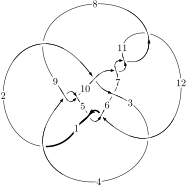
\includegraphics[width=112pt]{../../../GIT/diagram.site/Diagrams/png/2002_12a_1201.png}\\
\ \ \ A knot diagram\footnotemark}&
\allowdisplaybreaks
\textbf{Linearized knot diagam} \\
\cline{2-2}
 &
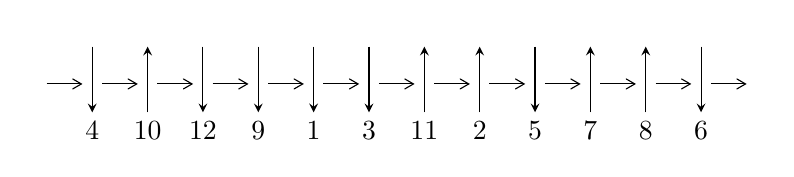
\begin{tikzpicture}[x=20pt, y=17pt]
	% nodes
	\node (C0) at (0, 0) {};
	\node (C1) at (1, 0) {};
	\node (C1U) at (1, +1) {};
	\node (C1D) at (1, -1) {4};

	\node (C2) at (2, 0) {};
	\node (C2U) at (2, +1) {};
	\node (C2D) at (2, -1) {10};

	\node (C3) at (3, 0) {};
	\node (C3U) at (3, +1) {};
	\node (C3D) at (3, -1) {12};

	\node (C4) at (4, 0) {};
	\node (C4U) at (4, +1) {};
	\node (C4D) at (4, -1) {9};

	\node (C5) at (5, 0) {};
	\node (C5U) at (5, +1) {};
	\node (C5D) at (5, -1) {1};

	\node (C6) at (6, 0) {};
	\node (C6U) at (6, +1) {};
	\node (C6D) at (6, -1) {3};

	\node (C7) at (7, 0) {};
	\node (C7U) at (7, +1) {};
	\node (C7D) at (7, -1) {11};

	\node (C8) at (8, 0) {};
	\node (C8U) at (8, +1) {};
	\node (C8D) at (8, -1) {2};

	\node (C9) at (9, 0) {};
	\node (C9U) at (9, +1) {};
	\node (C9D) at (9, -1) {5};

	\node (C10) at (10, 0) {};
	\node (C10U) at (10, +1) {};
	\node (C10D) at (10, -1) {7};

	\node (C11) at (11, 0) {};
	\node (C11U) at (11, +1) {};
	\node (C11D) at (11, -1) {8};

	\node (C12) at (12, 0) {};
	\node (C12U) at (12, +1) {};
	\node (C12D) at (12, -1) {6};
	\node (C13) at (13, 0) {};

	% arrows
	\draw[->,>={angle 60}]
	(C0) edge (C1) (C1) edge (C2) (C2) edge (C3) (C3) edge (C4) (C4) edge (C5) (C5) edge (C6) (C6) edge (C7) (C7) edge (C8) (C8) edge (C9) (C9) edge (C10) (C10) edge (C11) (C11) edge (C12) (C12) edge (C13) ;	\draw[->,>=stealth]
	(C1U) edge (C1D) (C2D) edge (C2U) (C3U) edge (C3D) (C4U) edge (C4D) (C5U) edge (C5D) (C6U) edge (C6D) (C7D) edge (C7U) (C8D) edge (C8U) (C9U) edge (C9D) (C10D) edge (C10U) (C11D) edge (C11U) (C12U) edge (C12D) ;
	\end{tikzpicture} \\
\hhline{~~} \\& 
\textbf{Solving Sequence} \\ \cline{2-2} 
 &
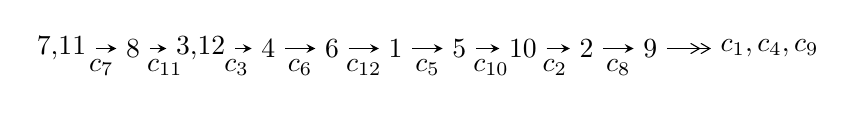
\begin{tikzpicture}[x=23pt, y=7pt]
	% node
	\node (A0) at (-1/8, 0) {7,11};
	\node (A1) at (1, 0) {8};
	\node (A2) at (33/16, 0) {3,12};
	\node (A3) at (25/8, 0) {4};
	\node (A4) at (33/8, 0) {6};
	\node (A5) at (41/8, 0) {1};
	\node (A6) at (49/8, 0) {5};
	\node (A7) at (57/8, 0) {10};
	\node (A8) at (65/8, 0) {2};
	\node (A9) at (73/8, 0) {9};
	\node (C1) at (1/2, -1) {$c_{7}$};
	\node (C2) at (3/2, -1) {$c_{11}$};
	\node (C3) at (21/8, -1) {$c_{3}$};
	\node (C4) at (29/8, -1) {$c_{6}$};
	\node (C5) at (37/8, -1) {$c_{12}$};
	\node (C6) at (45/8, -1) {$c_{5}$};
	\node (C7) at (53/8, -1) {$c_{10}$};
	\node (C8) at (61/8, -1) {$c_{2}$};
	\node (C9) at (69/8, -1) {$c_{8}$};
	\node (A10) at (11, 0) {$c_{1},c_{4},c_{9}$};

	% edge
	\draw[->,>=stealth]	
	(A0) edge (A1) (A1) edge (A2) (A2) edge (A3) (A3) edge (A4) (A4) edge (A5) (A5) edge (A6) (A6) edge (A7) (A7) edge (A8) (A8) edge (A9) ;
	\draw[->>,>={angle 60}]	
	(A9) edge (A10);
\end{tikzpicture} \\ 

\end{tabular} \\

\footnotetext{
The image of knot diagram is generated by the software ``\textbf{Draw programme}" developed by Andrew Bartholomew(\url{http://www.layer8.co.uk/maths/draw/index.htm\#Running-draw}), where we modified some parts for our purpose(\url{https://github.com/CATsTAILs/LinksPainter}).
}\phantom \\ \newline 
\centering \textbf{Ideals for irreducible components\footnotemark of $X_{\text{par}}$} 
 
\begin{align*}
I^u_{1}&=\langle 
-4.70258\times10^{345} u^{139}+1.45980\times10^{346} u^{138}+\cdots+2.18893\times10^{345} b+3.04112\times10^{346},\\
\phantom{I^u_{1}}&\phantom{= \langle  }3.74652\times10^{346} u^{139}-1.17909\times10^{347} u^{138}+\cdots+2.18893\times10^{345} a-1.90043\times10^{347},\\
\phantom{I^u_{1}}&\phantom{= \langle  }u^{140}-3 u^{139}+\cdots-27 u-1\rangle \\
I^u_{2}&=\langle 
-286723 u^{34}+444928 u^{33}+\cdots+69517 b+453427,\\
\phantom{I^u_{2}}&\phantom{= \langle  }8945075 u^{34}-15497918 u^{33}+\cdots+69517 a-7160101,\;u^{35}-3 u^{34}+\cdots-3 u+1\rangle \\
I^u_{3}&=\langle 
b-1,\;a,\;u-1\rangle \\
\\
\end{align*}
\raggedright * 3 irreducible components of $\dim_{\mathbb{C}}=0$, with total 176 representations.\\
\footnotetext{All coefficients of polynomials are rational numbers. But the coefficients are sometimes approximated in decimal forms when there is not enough margin.}
\newpage
\renewcommand{\arraystretch}{1}
\centering \section*{I. $I^u_{1}= \langle -4.70\times10^{345} u^{139}+1.46\times10^{346} u^{138}+\cdots+2.19\times10^{345} b+3.04\times10^{346},\;3.75\times10^{346} u^{139}-1.18\times10^{347} u^{138}+\cdots+2.19\times10^{345} a-1.90\times10^{347},\;u^{140}-3 u^{139}+\cdots-27 u-1 \rangle$}
\flushleft \textbf{(i) Arc colorings}\\
\begin{tabular}{m{7pt} m{180pt} m{7pt} m{180pt} }
\flushright $a_{7}=$&$\begin{pmatrix}1\\0\end{pmatrix}$ \\
\flushright $a_{11}=$&$\begin{pmatrix}0\\u\end{pmatrix}$ \\
\flushright $a_{8}=$&$\begin{pmatrix}1\\- u^2\end{pmatrix}$ \\
\flushright $a_{3}=$&$\begin{pmatrix}-17.1157 u^{139}+53.8661 u^{138}+\cdots+1840.02 u+86.8198\\2.14834 u^{139}-6.66899 u^{138}+\cdots-278.821 u-13.8932\end{pmatrix}$ \\
\flushright $a_{12}=$&$\begin{pmatrix}u\\- u^3+u\end{pmatrix}$ \\
\flushright $a_{4}=$&$\begin{pmatrix}-17.4779 u^{139}+55.4038 u^{138}+\cdots+1913.85 u+90.1905\\1.24479 u^{139}-4.12684 u^{138}+\cdots-216.821 u-10.9738\end{pmatrix}$ \\
\flushright $a_{6}=$&$\begin{pmatrix}-2.34681 u^{139}+4.30372 u^{138}+\cdots+657.341 u+40.8192\\2.78708 u^{139}-6.59659 u^{138}+\cdots-259.251 u-13.1983\end{pmatrix}$ \\
\flushright $a_{1}=$&$\begin{pmatrix}-15.4483 u^{139}+49.0551 u^{138}+\cdots+2205.24 u+104.962\\1.59584 u^{139}-6.60896 u^{138}+\cdots-250.220 u-12.3168\end{pmatrix}$ \\
\flushright $a_{5}=$&$\begin{pmatrix}-13.4458 u^{139}+41.6387 u^{138}+\cdots+1644.46 u+82.0808\\2.89425 u^{139}-7.86046 u^{138}+\cdots-350.112 u-16.8488\end{pmatrix}$ \\
\flushright $a_{10}=$&$\begin{pmatrix}- u\\u\end{pmatrix}$ \\
\flushright $a_{2}=$&$\begin{pmatrix}-15.8887 u^{139}+50.8414 u^{138}+\cdots+1793.03 u+84.5248\\0.921328 u^{139}-3.64428 u^{138}+\cdots-231.824 u-11.5982\end{pmatrix}$ \\
\flushright $a_{9}=$&$\begin{pmatrix}-4.06898 u^{139}+13.2143 u^{138}+\cdots+1095.07 u+58.9998\\1.75915 u^{139}-6.31156 u^{138}+\cdots-361.334 u-16.8026\end{pmatrix}$\\&\end{tabular}
\flushleft \textbf{(ii) Obstruction class $= -1$}\\~\\
\flushleft \textbf{(iii) Cusp Shapes $= 28.6964 u^{139}-93.7293 u^{138}+\cdots-3097.74 u-147.900$}\\~\\
\newpage\renewcommand{\arraystretch}{1}
\flushleft \textbf{(iv) u-Polynomials at the component}\newline \\
\begin{tabular}{m{50pt}|m{274pt}}
Crossings & \hspace{64pt}u-Polynomials at each crossing \\
\hline $$\begin{aligned}c_{1}\end{aligned}$$&$\begin{aligned}
&u^{140}+u^{139}+\cdots+405 u+119
\end{aligned}$\\
\hline $$\begin{aligned}c_{2}\end{aligned}$$&$\begin{aligned}
&u^{140}+4 u^{139}+\cdots+44695798 u-3369031
\end{aligned}$\\
\hline $$\begin{aligned}c_{3}\end{aligned}$$&$\begin{aligned}
&u^{140}-4 u^{139}+\cdots-29465412 u+1871711
\end{aligned}$\\
\hline $$\begin{aligned}c_{4},c_{9}\end{aligned}$$&$\begin{aligned}
&u^{140}-2 u^{139}+\cdots-8527 u+2089
\end{aligned}$\\
\hline $$\begin{aligned}c_{5},c_{12}\end{aligned}$$&$\begin{aligned}
&u^{140}+3 u^{139}+\cdots+63834 u-5809
\end{aligned}$\\
\hline $$\begin{aligned}c_{6}\end{aligned}$$&$\begin{aligned}
&u^{140}+7 u^{139}+\cdots+208242066 u-166275911
\end{aligned}$\\
\hline $$\begin{aligned}c_{7},c_{10},c_{11}\end{aligned}$$&$\begin{aligned}
&u^{140}-3 u^{139}+\cdots-27 u-1
\end{aligned}$\\
\hline $$\begin{aligned}c_{8}\end{aligned}$$&$\begin{aligned}
&u^{140}+15 u^{138}+\cdots+315207 u-35883
\end{aligned}$\\
\hline
\end{tabular}\\~\\
\newpage\renewcommand{\arraystretch}{1}
\flushleft \textbf{(v) Riley Polynomials at the component}\newline \\
\begin{tabular}{m{50pt}|m{274pt}}
Crossings & \hspace{64pt}Riley Polynomials at each crossing \\
\hline $$\begin{aligned}c_{1}\end{aligned}$$&$\begin{aligned}
&y^{140}-5 y^{139}+\cdots+6830319 y+14161
\end{aligned}$\\
\hline $$\begin{aligned}c_{2}\end{aligned}$$&$\begin{aligned}
&y^{140}-34 y^{139}+\cdots-510524756422924 y+11350369878961
\end{aligned}$\\
\hline $$\begin{aligned}c_{3}\end{aligned}$$&$\begin{aligned}
&y^{140}+56 y^{139}+\cdots+52970751482880 y+3503302067521
\end{aligned}$\\
\hline $$\begin{aligned}c_{4},c_{9}\end{aligned}$$&$\begin{aligned}
&y^{140}-74 y^{139}+\cdots-86881505 y+4363921
\end{aligned}$\\
\hline $$\begin{aligned}c_{5},c_{12}\end{aligned}$$&$\begin{aligned}
&y^{140}+105 y^{139}+\cdots+2341783754 y+33744481
\end{aligned}$\\
\hline $$\begin{aligned}c_{6}\end{aligned}$$&$\begin{aligned}
&y^{140}+57 y^{139}+\cdots+1894560234749566132 y+27647678578879921
\end{aligned}$\\
\hline $$\begin{aligned}c_{7},c_{10},c_{11}\end{aligned}$$&$\begin{aligned}
&y^{140}-139 y^{139}+\cdots-63 y+1
\end{aligned}$\\
\hline $$\begin{aligned}c_{8}\end{aligned}$$&$\begin{aligned}
&y^{140}+30 y^{139}+\cdots+67712278617 y+1287589689
\end{aligned}$\\
\hline
\end{tabular}\\~\\
\newpage\flushleft \textbf{(vi) Complex Volumes and Cusp Shapes}
$$\begin{array}{c|c|c}  
\text{Solutions to }I^u_{1}& \I (\text{vol} + \sqrt{-1}CS) & \text{Cusp shape}\\
 \hline 
\begin{aligned}
u &= -0.462379 + 0.872851 I \\
a &= \phantom{-}0.457037 - 0.280992 I \\
b &= \phantom{-}0.668404 + 0.884753 I\end{aligned}
 & -3.71972 - 8.53606 I & \phantom{-0.000000 } 0 \\ \hline\begin{aligned}
u &= -0.462379 - 0.872851 I \\
a &= \phantom{-}0.457037 + 0.280992 I \\
b &= \phantom{-}0.668404 - 0.884753 I\end{aligned}
 & -3.71972 + 8.53606 I & \phantom{-0.000000 } 0 \\ \hline\begin{aligned}
u &= -0.704341 + 0.737453 I \\
a &= \phantom{-}0.776491 - 0.006136 I \\
b &= -0.504752 + 1.084340 I\end{aligned}
 & \phantom{-}1.77897 + 9.64332 I & \phantom{-0.000000 } 0 \\ \hline\begin{aligned}
u &= -0.704341 - 0.737453 I \\
a &= \phantom{-}0.776491 + 0.006136 I \\
b &= -0.504752 - 1.084340 I\end{aligned}
 & \phantom{-}1.77897 - 9.64332 I & \phantom{-0.000000 } 0 \\ \hline\begin{aligned}
u &= \phantom{-}0.686254 + 0.756748 I \\
a &= -0.715275 - 0.188941 I \\
b &= \phantom{-}0.395128 + 0.982604 I\end{aligned}
 & \phantom{-}4.72890 - 3.27964 I & \phantom{-0.000000 } 0 \\ \hline\begin{aligned}
u &= \phantom{-}0.686254 - 0.756748 I \\
a &= -0.715275 + 0.188941 I \\
b &= \phantom{-}0.395128 - 0.982604 I\end{aligned}
 & \phantom{-}4.72890 + 3.27964 I & \phantom{-0.000000 } 0 \\ \hline\begin{aligned}
u &= \phantom{-}0.377083 + 0.883614 I \\
a &= \phantom{-}0.539975 - 0.407438 I \\
b &= -0.046896 - 0.826372 I\end{aligned}
 & \phantom{-}2.01560 - 1.61773 I & \phantom{-0.000000 } 0 \\ \hline\begin{aligned}
u &= \phantom{-}0.377083 - 0.883614 I \\
a &= \phantom{-}0.539975 + 0.407438 I \\
b &= -0.046896 + 0.826372 I\end{aligned}
 & \phantom{-}2.01560 + 1.61773 I & \phantom{-0.000000 } 0 \\ \hline\begin{aligned}
u &= \phantom{-}0.478507 + 0.828531 I \\
a &= \phantom{-}0.577416 + 0.614164 I \\
b &= \phantom{-}0.667428 - 1.197920 I\end{aligned}
 & \phantom{-}4.12877 + 8.61622 I & \phantom{-0.000000 } 0 \\ \hline\begin{aligned}
u &= \phantom{-}0.478507 - 0.828531 I \\
a &= \phantom{-}0.577416 - 0.614164 I \\
b &= \phantom{-}0.667428 + 1.197920 I\end{aligned}
 & \phantom{-}4.12877 - 8.61622 I & \phantom{-0.000000 } 0\\
 \hline 
 \end{array}$$\newpage$$\begin{array}{c|c|c}  
\text{Solutions to }I^u_{1}& \I (\text{vol} + \sqrt{-1}CS) & \text{Cusp shape}\\
 \hline 
\begin{aligned}
u &= -0.456133 + 0.833311 I \\
a &= -0.674185 + 0.539381 I \\
b &= -0.80454 - 1.28700 I\end{aligned}
 & \phantom{-}1.0425 - 14.9384 I & \phantom{-0.000000 } 0 \\ \hline\begin{aligned}
u &= -0.456133 - 0.833311 I \\
a &= -0.674185 - 0.539381 I \\
b &= -0.80454 + 1.28700 I\end{aligned}
 & \phantom{-}1.0425 + 14.9384 I & \phantom{-0.000000 } 0 \\ \hline\begin{aligned}
u &= \phantom{-}0.964246 + 0.434277 I \\
a &= \phantom{-}0.562867 + 0.368503 I \\
b &= -0.137014 - 0.528866 I\end{aligned}
 & \phantom{-}1.46755 + 0.80554 I & \phantom{-0.000000 } 0 \\ \hline\begin{aligned}
u &= \phantom{-}0.964246 - 0.434277 I \\
a &= \phantom{-}0.562867 - 0.368503 I \\
b &= -0.137014 + 0.528866 I\end{aligned}
 & \phantom{-}1.46755 - 0.80554 I & \phantom{-0.000000 } 0 \\ \hline\begin{aligned}
u &= -0.328180 + 0.878078 I \\
a &= \phantom{-}0.354828 - 0.320483 I \\
b &= \phantom{-}0.309412 + 0.571510 I\end{aligned}
 & -3.62334 + 1.06275 I & \phantom{-0.000000 } 0 \\ \hline\begin{aligned}
u &= -0.328180 - 0.878078 I \\
a &= \phantom{-}0.354828 + 0.320483 I \\
b &= \phantom{-}0.309412 - 0.571510 I\end{aligned}
 & -3.62334 - 1.06275 I & \phantom{-0.000000 } 0 \\ \hline\begin{aligned}
u &= \phantom{-}0.403616 + 0.815553 I \\
a &= -0.425989 - 0.236906 I \\
b &= -0.456070 + 0.937118 I\end{aligned}
 & \phantom{-}0.10647 + 3.89798 I & \phantom{-0.000000 } 0 \\ \hline\begin{aligned}
u &= \phantom{-}0.403616 - 0.815553 I \\
a &= -0.425989 + 0.236906 I \\
b &= -0.456070 - 0.937118 I\end{aligned}
 & \phantom{-}0.10647 - 3.89798 I & \phantom{-0.000000 } 0 \\ \hline\begin{aligned}
u &= -0.170842 + 0.884336 I \\
a &= -0.458227 - 0.527772 I \\
b &= \phantom{-}0.006089 - 0.657947 I\end{aligned}
 & \phantom{-}1.93663 - 0.61257 I & \phantom{-0.000000 } 0 \\ \hline\begin{aligned}
u &= -0.170842 - 0.884336 I \\
a &= -0.458227 + 0.527772 I \\
b &= \phantom{-}0.006089 + 0.657947 I\end{aligned}
 & \phantom{-}1.93663 + 0.61257 I & \phantom{-0.000000 } 0\\
 \hline 
 \end{array}$$\newpage$$\begin{array}{c|c|c}  
\text{Solutions to }I^u_{1}& \I (\text{vol} + \sqrt{-1}CS) & \text{Cusp shape}\\
 \hline 
\begin{aligned}
u &= -0.818840 + 0.775513 I \\
a &= -0.418165 - 0.019733 I \\
b &= \phantom{-}0.167714 - 0.698294 I\end{aligned}
 & -2.76939 + 2.90326 I & \phantom{-0.000000 } 0 \\ \hline\begin{aligned}
u &= -0.818840 - 0.775513 I \\
a &= -0.418165 + 0.019733 I \\
b &= \phantom{-}0.167714 + 0.698294 I\end{aligned}
 & -2.76939 - 2.90326 I & \phantom{-0.000000 } 0 \\ \hline\begin{aligned}
u &= \phantom{-}0.623465 + 0.592662 I \\
a &= -0.355432 - 0.388206 I \\
b &= -0.666980 + 1.179240 I\end{aligned}
 & \phantom{-}3.08454 + 6.40753 I & \phantom{-0.000000 } 0 \\ \hline\begin{aligned}
u &= \phantom{-}0.623465 - 0.592662 I \\
a &= -0.355432 + 0.388206 I \\
b &= -0.666980 - 1.179240 I\end{aligned}
 & \phantom{-}3.08454 - 6.40753 I & \phantom{-0.000000 } 0 \\ \hline\begin{aligned}
u &= -1.136100 + 0.122033 I \\
a &= -0.434683 + 0.268499 I \\
b &= \phantom{-}0.804708 + 0.523340 I\end{aligned}
 & \phantom{-}4.56061 - 3.17341 I & \phantom{-0.000000 } 0 \\ \hline\begin{aligned}
u &= -1.136100 - 0.122033 I \\
a &= -0.434683 - 0.268499 I \\
b &= \phantom{-}0.804708 - 0.523340 I\end{aligned}
 & \phantom{-}4.56061 + 3.17341 I & \phantom{-0.000000 } 0 \\ \hline\begin{aligned}
u &= \phantom{-}1.16073\phantom{ +0.000000I} \\
a &= \phantom{-}0.0578993\phantom{ +0.000000I} \\
b &= \phantom{-}1.04319\phantom{ +0.000000I}\end{aligned}
 & -1.61847\phantom{ +0.000000I} & \phantom{-0.000000 } 0 \\ \hline\begin{aligned}
u &= -0.465931 + 0.682708 I \\
a &= -0.715701 + 0.938995 I \\
b &= -0.735843 - 0.794635 I\end{aligned}
 & -2.80541 - 4.22675 I & \phantom{-0.000000 } 0 \\ \hline\begin{aligned}
u &= -0.465931 - 0.682708 I \\
a &= -0.715701 - 0.938995 I \\
b &= -0.735843 + 0.794635 I\end{aligned}
 & -2.80541 + 4.22675 I & \phantom{-0.000000 } 0 \\ \hline\begin{aligned}
u &= \phantom{-}0.805832 + 0.171888 I \\
a &= -0.72972 + 1.84695 I \\
b &= \phantom{-}0.542835 - 0.558432 I\end{aligned}
 & \phantom{-}3.36428 + 0.17780 I & \phantom{-0.000000 } 0\\
 \hline 
 \end{array}$$\newpage$$\begin{array}{c|c|c}  
\text{Solutions to }I^u_{1}& \I (\text{vol} + \sqrt{-1}CS) & \text{Cusp shape}\\
 \hline 
\begin{aligned}
u &= \phantom{-}0.805832 - 0.171888 I \\
a &= -0.72972 - 1.84695 I \\
b &= \phantom{-}0.542835 + 0.558432 I\end{aligned}
 & \phantom{-}3.36428 - 0.17780 I & \phantom{-0.000000 } 0 \\ \hline\begin{aligned}
u &= -0.631596 + 0.501522 I \\
a &= \phantom{-}0.293717 + 0.046531 I \\
b &= -0.684176 + 0.529370 I\end{aligned}
 & -2.30853 + 0.01280 I & \phantom{-0.000000 } 0 \\ \hline\begin{aligned}
u &= -0.631596 - 0.501522 I \\
a &= \phantom{-}0.293717 - 0.046531 I \\
b &= -0.684176 - 0.529370 I\end{aligned}
 & -2.30853 - 0.01280 I & \phantom{-0.000000 } 0 \\ \hline\begin{aligned}
u &= -1.217270 + 0.004425 I \\
a &= \phantom{-}1.30064 - 2.33815 I \\
b &= -1.07297 + 1.32920 I\end{aligned}
 & \phantom{-}1.04242 - 5.47669 I & \phantom{-0.000000 } 0 \\ \hline\begin{aligned}
u &= -1.217270 - 0.004425 I \\
a &= \phantom{-}1.30064 + 2.33815 I \\
b &= -1.07297 - 1.32920 I\end{aligned}
 & \phantom{-}1.04242 + 5.47669 I & \phantom{-0.000000 } 0 \\ \hline\begin{aligned}
u &= \phantom{-}0.601253 + 0.469515 I \\
a &= \phantom{-}0.759163 + 0.277979 I \\
b &= \phantom{-}0.183519 - 0.606937 I\end{aligned}
 & \phantom{-}1.29364 + 0.77209 I & \phantom{-0.000000 } 0 \\ \hline\begin{aligned}
u &= \phantom{-}0.601253 - 0.469515 I \\
a &= \phantom{-}0.759163 - 0.277979 I \\
b &= \phantom{-}0.183519 + 0.606937 I\end{aligned}
 & \phantom{-}1.29364 - 0.77209 I & \phantom{-0.000000 } 0 \\ \hline\begin{aligned}
u &= -1.070230 + 0.636332 I \\
a &= -0.092737 + 0.241677 I \\
b &= \phantom{-}0.134547 - 0.437874 I\end{aligned}
 & -1.48417 - 6.45366 I & \phantom{-0.000000 } 0 \\ \hline\begin{aligned}
u &= -1.070230 - 0.636332 I \\
a &= -0.092737 - 0.241677 I \\
b &= \phantom{-}0.134547 + 0.437874 I\end{aligned}
 & -1.48417 + 6.45366 I & \phantom{-0.000000 } 0 \\ \hline\begin{aligned}
u &= \phantom{-}0.398072 + 0.626175 I \\
a &= -0.946969 - 0.318541 I \\
b &= -0.79762 + 1.43794 I\end{aligned}
 & \phantom{-}2.96797 + 2.33819 I & \phantom{-0.000000 } 0\\
 \hline 
 \end{array}$$\newpage$$\begin{array}{c|c|c}  
\text{Solutions to }I^u_{1}& \I (\text{vol} + \sqrt{-1}CS) & \text{Cusp shape}\\
 \hline 
\begin{aligned}
u &= \phantom{-}0.398072 - 0.626175 I \\
a &= -0.946969 + 0.318541 I \\
b &= -0.79762 - 1.43794 I\end{aligned}
 & \phantom{-}2.96797 - 2.33819 I & \phantom{-0.000000 } 0 \\ \hline\begin{aligned}
u &= \phantom{-}1.241780 + 0.220632 I \\
a &= -0.90441 - 1.62834 I \\
b &= \phantom{-}0.609759 + 1.255110 I\end{aligned}
 & \phantom{-}2.80271 + 0.23073 I & \phantom{-0.000000 } 0 \\ \hline\begin{aligned}
u &= \phantom{-}1.241780 - 0.220632 I \\
a &= -0.90441 + 1.62834 I \\
b &= \phantom{-}0.609759 - 1.255110 I\end{aligned}
 & \phantom{-}2.80271 - 0.23073 I & \phantom{-0.000000 } 0 \\ \hline\begin{aligned}
u &= \phantom{-}1.260930 + 0.082460 I \\
a &= \phantom{-}0.086207 - 0.530918 I \\
b &= -1.184450 - 0.384164 I\end{aligned}
 & \phantom{-}2.27831 - 4.47551 I & \phantom{-0.000000 } 0 \\ \hline\begin{aligned}
u &= \phantom{-}1.260930 - 0.082460 I \\
a &= \phantom{-}0.086207 + 0.530918 I \\
b &= -1.184450 + 0.384164 I\end{aligned}
 & \phantom{-}2.27831 + 4.47551 I & \phantom{-0.000000 } 0 \\ \hline\begin{aligned}
u &= -1.315690 + 0.009991 I \\
a &= -0.36004 - 2.74746 I \\
b &= \phantom{-}0.05423 + 1.82083 I\end{aligned}
 & \phantom{-}0.10570 + 2.10964 I & \phantom{-0.000000 } 0 \\ \hline\begin{aligned}
u &= -1.315690 - 0.009991 I \\
a &= -0.36004 + 2.74746 I \\
b &= \phantom{-}0.05423 - 1.82083 I\end{aligned}
 & \phantom{-}0.10570 - 2.10964 I & \phantom{-0.000000 } 0 \\ \hline\begin{aligned}
u &= -1.313990 + 0.111074 I \\
a &= -0.23144 - 1.79391 I \\
b &= \phantom{-}0.031189 + 0.365803 I\end{aligned}
 & -0.70589 - 4.44648 I & \phantom{-0.000000 } 0 \\ \hline\begin{aligned}
u &= -1.313990 - 0.111074 I \\
a &= -0.23144 + 1.79391 I \\
b &= \phantom{-}0.031189 - 0.365803 I\end{aligned}
 & -0.70589 + 4.44648 I & \phantom{-0.000000 } 0 \\ \hline\begin{aligned}
u &= \phantom{-}0.423118 + 0.522894 I \\
a &= \phantom{-}1.237050 - 0.528772 I \\
b &= -0.158698 - 1.136510 I\end{aligned}
 & \phantom{-}3.23668 + 1.44238 I & \phantom{-0.000000 } 0\\
 \hline 
 \end{array}$$\newpage$$\begin{array}{c|c|c}  
\text{Solutions to }I^u_{1}& \I (\text{vol} + \sqrt{-1}CS) & \text{Cusp shape}\\
 \hline 
\begin{aligned}
u &= \phantom{-}0.423118 - 0.522894 I \\
a &= \phantom{-}1.237050 + 0.528772 I \\
b &= -0.158698 + 1.136510 I\end{aligned}
 & \phantom{-}3.23668 - 1.44238 I & \phantom{-0.000000 } 0 \\ \hline\begin{aligned}
u &= -0.129908 + 0.651480 I \\
a &= \phantom{-}0.133831 + 0.582906 I \\
b &= \phantom{-}0.060763 - 1.345760 I\end{aligned}
 & -1.41806 + 3.01802 I & \phantom{-0.000000 } 0 \\ \hline\begin{aligned}
u &= -0.129908 - 0.651480 I \\
a &= \phantom{-}0.133831 - 0.582906 I \\
b &= \phantom{-}0.060763 + 1.345760 I\end{aligned}
 & -1.41806 - 3.01802 I & \phantom{-0.000000 } 0 \\ \hline\begin{aligned}
u &= -0.565129 + 0.345483 I \\
a &= -0.086280 - 0.838713 I \\
b &= \phantom{-}0.699439 + 1.051320 I\end{aligned}
 & \phantom{-}4.07356 - 3.29083 I & \phantom{-0.000000 } 0 \\ \hline\begin{aligned}
u &= -0.565129 - 0.345483 I \\
a &= -0.086280 + 0.838713 I \\
b &= \phantom{-}0.699439 - 1.051320 I\end{aligned}
 & \phantom{-}4.07356 + 3.29083 I & \phantom{-0.000000 } 0 \\ \hline\begin{aligned}
u &= \phantom{-}1.329060 + 0.180992 I \\
a &= \phantom{-}1.162230 + 0.506902 I \\
b &= -1.107950 - 0.567617 I\end{aligned}
 & \phantom{-}2.37634 + 1.48237 I & \phantom{-0.000000 } 0 \\ \hline\begin{aligned}
u &= \phantom{-}1.329060 - 0.180992 I \\
a &= \phantom{-}1.162230 - 0.506902 I \\
b &= -1.107950 + 0.567617 I\end{aligned}
 & \phantom{-}2.37634 - 1.48237 I & \phantom{-0.000000 } 0 \\ \hline\begin{aligned}
u &= \phantom{-}1.343570 + 0.059602 I \\
a &= \phantom{-}0.17148 - 1.95113 I \\
b &= -0.017383 + 1.108000 I\end{aligned}
 & \phantom{-}3.06942 + 1.61488 I & \phantom{-0.000000 } 0 \\ \hline\begin{aligned}
u &= \phantom{-}1.343570 - 0.059602 I \\
a &= \phantom{-}0.17148 + 1.95113 I \\
b &= -0.017383 - 1.108000 I\end{aligned}
 & \phantom{-}3.06942 - 1.61488 I & \phantom{-0.000000 } 0 \\ \hline\begin{aligned}
u &= -0.320764 + 0.569441 I \\
a &= \phantom{-}1.31405 - 0.73024 I \\
b &= \phantom{-}1.08104 + 1.24019 I\end{aligned}
 & \phantom{-}3.26804 - 5.06148 I & \phantom{-0.000000 } 0\\
 \hline 
 \end{array}$$\newpage$$\begin{array}{c|c|c}  
\text{Solutions to }I^u_{1}& \I (\text{vol} + \sqrt{-1}CS) & \text{Cusp shape}\\
 \hline 
\begin{aligned}
u &= -0.320764 - 0.569441 I \\
a &= \phantom{-}1.31405 + 0.73024 I \\
b &= \phantom{-}1.08104 - 1.24019 I\end{aligned}
 & \phantom{-}3.26804 + 5.06148 I & \phantom{-0.000000 } 0 \\ \hline\begin{aligned}
u &= -0.425132 + 0.490297 I \\
a &= -1.53497 + 0.84982 I \\
b &= -0.674783 - 0.719553 I\end{aligned}
 & -1.89546 - 4.32229 I & \phantom{-0.000000 } 0 \\ \hline\begin{aligned}
u &= -0.425132 - 0.490297 I \\
a &= -1.53497 - 0.84982 I \\
b &= -0.674783 + 0.719553 I\end{aligned}
 & -1.89546 + 4.32229 I & \phantom{-0.000000 } 0 \\ \hline\begin{aligned}
u &= -0.560763 + 0.315780 I \\
a &= \phantom{-}2.53851 - 1.29915 I \\
b &= -0.154600 + 0.718380 I\end{aligned}
 & \phantom{-}0.39792 - 6.14230 I & \phantom{-0.000000 -}0. + 8.00126 I \\ \hline\begin{aligned}
u &= -0.560763 - 0.315780 I \\
a &= \phantom{-}2.53851 + 1.29915 I \\
b &= -0.154600 - 0.718380 I\end{aligned}
 & \phantom{-}0.39792 + 6.14230 I & \phantom{-0.000000 } 0. - 8.00126 I \\ \hline\begin{aligned}
u &= -1.359650 + 0.117728 I \\
a &= -1.105820 - 0.418584 I \\
b &= \phantom{-}1.69043 + 0.21809 I\end{aligned}
 & \phantom{-}5.88239 - 4.59774 I & \phantom{-0.000000 } 0 \\ \hline\begin{aligned}
u &= -1.359650 - 0.117728 I \\
a &= -1.105820 + 0.418584 I \\
b &= \phantom{-}1.69043 - 0.21809 I\end{aligned}
 & \phantom{-}5.88239 + 4.59774 I & \phantom{-0.000000 } 0 \\ \hline\begin{aligned}
u &= -1.362510 + 0.085272 I \\
a &= \phantom{-}0.43387 + 2.68486 I \\
b &= -0.568408 - 0.582435 I\end{aligned}
 & \phantom{-}2.91886 - 7.73986 I & \phantom{-0.000000 } 0 \\ \hline\begin{aligned}
u &= -1.362510 - 0.085272 I \\
a &= \phantom{-}0.43387 - 2.68486 I \\
b &= -0.568408 + 0.582435 I\end{aligned}
 & \phantom{-}2.91886 + 7.73986 I & \phantom{-0.000000 } 0 \\ \hline\begin{aligned}
u &= -1.372620 + 0.041492 I \\
a &= \phantom{-}0.910453 - 0.463763 I \\
b &= -1.62467 + 0.42421 I\end{aligned}
 & \phantom{-}2.97120 - 0.46899 I & \phantom{-0.000000 } 0\\
 \hline 
 \end{array}$$\newpage$$\begin{array}{c|c|c}  
\text{Solutions to }I^u_{1}& \I (\text{vol} + \sqrt{-1}CS) & \text{Cusp shape}\\
 \hline 
\begin{aligned}
u &= -1.372620 - 0.041492 I \\
a &= \phantom{-}0.910453 + 0.463763 I \\
b &= -1.62467 - 0.42421 I\end{aligned}
 & \phantom{-}2.97120 + 0.46899 I & \phantom{-0.000000 } 0 \\ \hline\begin{aligned}
u &= \phantom{-}1.381760 + 0.136726 I \\
a &= \phantom{-}1.72384 - 0.47772 I \\
b &= -2.23547 - 0.03375 I\end{aligned}
 & \phantom{-}3.20477 + 9.15153 I & \phantom{-0.000000 } 0 \\ \hline\begin{aligned}
u &= \phantom{-}1.381760 - 0.136726 I \\
a &= \phantom{-}1.72384 + 0.47772 I \\
b &= -2.23547 + 0.03375 I\end{aligned}
 & \phantom{-}3.20477 - 9.15153 I & \phantom{-0.000000 } 0 \\ \hline\begin{aligned}
u &= \phantom{-}1.376280 + 0.254400 I \\
a &= -1.28784 - 1.04043 I \\
b &= \phantom{-}0.209891 + 1.329590 I\end{aligned}
 & \phantom{-}8.43189 + 0.58347 I & \phantom{-0.000000 } 0 \\ \hline\begin{aligned}
u &= \phantom{-}1.376280 - 0.254400 I \\
a &= -1.28784 + 1.04043 I \\
b &= \phantom{-}0.209891 - 1.329590 I\end{aligned}
 & \phantom{-}8.43189 - 0.58347 I & \phantom{-0.000000 } 0 \\ \hline\begin{aligned}
u &= \phantom{-}1.400760 + 0.095179 I \\
a &= -1.14022 - 1.06949 I \\
b &= \phantom{-}1.62050 + 1.13483 I\end{aligned}
 & \phantom{-}1.58883 + 4.27435 I & \phantom{-0.000000 } 0 \\ \hline\begin{aligned}
u &= \phantom{-}1.400760 - 0.095179 I \\
a &= -1.14022 + 1.06949 I \\
b &= \phantom{-}1.62050 - 1.13483 I\end{aligned}
 & \phantom{-}1.58883 - 4.27435 I & \phantom{-0.000000 } 0 \\ \hline\begin{aligned}
u &= -1.406880 + 0.006416 I \\
a &= \phantom{-}0.464909 - 1.094690 I \\
b &= \phantom{-}0.772828 + 0.884649 I\end{aligned}
 & \phantom{-}7.98154 - 2.83433 I & \phantom{-0.000000 } 0 \\ \hline\begin{aligned}
u &= -1.406880 - 0.006416 I \\
a &= \phantom{-}0.464909 + 1.094690 I \\
b &= \phantom{-}0.772828 - 0.884649 I\end{aligned}
 & \phantom{-}7.98154 + 2.83433 I & \phantom{-0.000000 } 0 \\ \hline\begin{aligned}
u &= -0.235792 + 0.542392 I \\
a &= -0.141507 + 0.081514 I \\
b &= -0.674308 + 0.917975 I\end{aligned}
 & -2.46402 + 1.20422 I & -4.02039 + 3.48565 I\\
 \hline 
 \end{array}$$\newpage$$\begin{array}{c|c|c}  
\text{Solutions to }I^u_{1}& \I (\text{vol} + \sqrt{-1}CS) & \text{Cusp shape}\\
 \hline 
\begin{aligned}
u &= -0.235792 - 0.542392 I \\
a &= -0.141507 - 0.081514 I \\
b &= -0.674308 - 0.917975 I\end{aligned}
 & -2.46402 - 1.20422 I & -4.02039 - 3.48565 I \\ \hline\begin{aligned}
u &= \phantom{-}1.42433 + 0.04690 I \\
a &= -0.84533 + 2.00807 I \\
b &= -0.056543 - 0.949934 I\end{aligned}
 & \phantom{-}8.82467 + 3.19321 I & \phantom{-0.000000 } 0 \\ \hline\begin{aligned}
u &= \phantom{-}1.42433 - 0.04690 I \\
a &= -0.84533 - 2.00807 I \\
b &= -0.056543 + 0.949934 I\end{aligned}
 & \phantom{-}8.82467 - 3.19321 I & \phantom{-0.000000 } 0 \\ \hline\begin{aligned}
u &= \phantom{-}1.42947 + 0.21457 I \\
a &= \phantom{-}0.00176 + 2.48122 I \\
b &= \phantom{-}1.23337 - 1.60979 I\end{aligned}
 & \phantom{-}8.90630 + 7.94848 I & \phantom{-0.000000 } 0 \\ \hline\begin{aligned}
u &= \phantom{-}1.42947 - 0.21457 I \\
a &= \phantom{-}0.00176 - 2.48122 I \\
b &= \phantom{-}1.23337 + 1.60979 I\end{aligned}
 & \phantom{-}8.90630 - 7.94848 I & \phantom{-0.000000 } 0 \\ \hline\begin{aligned}
u &= -1.43761 + 0.22669 I \\
a &= \phantom{-}0.76019 - 1.50877 I \\
b &= \phantom{-}0.40645 + 1.55265 I\end{aligned}
 & \phantom{-}9.06008 - 4.26529 I & \phantom{-0.000000 } 0 \\ \hline\begin{aligned}
u &= -1.43761 - 0.22669 I \\
a &= \phantom{-}0.76019 + 1.50877 I \\
b &= \phantom{-}0.40645 - 1.55265 I\end{aligned}
 & \phantom{-}9.06008 + 4.26529 I & \phantom{-0.000000 } 0 \\ \hline\begin{aligned}
u &= \phantom{-}0.140123 + 0.513834 I \\
a &= \phantom{-}0.435608 - 0.512064 I \\
b &= \phantom{-}1.100810 + 0.143302 I\end{aligned}
 & \phantom{-}1.21463 + 2.45922 I & -2.53647 - 5.18448 I \\ \hline\begin{aligned}
u &= \phantom{-}0.140123 - 0.513834 I \\
a &= \phantom{-}0.435608 + 0.512064 I \\
b &= \phantom{-}1.100810 - 0.143302 I\end{aligned}
 & \phantom{-}1.21463 - 2.45922 I & -2.53647 + 5.18448 I \\ \hline\begin{aligned}
u &= -1.45639 + 0.23069 I \\
a &= -0.23608 + 2.35336 I \\
b &= -1.00629 - 1.91711 I\end{aligned}
 & \phantom{-}8.94598 - 5.47573 I & \phantom{-0.000000 } 0\\
 \hline 
 \end{array}$$\newpage$$\begin{array}{c|c|c}  
\text{Solutions to }I^u_{1}& \I (\text{vol} + \sqrt{-1}CS) & \text{Cusp shape}\\
 \hline 
\begin{aligned}
u &= -1.45639 - 0.23069 I \\
a &= -0.23608 - 2.35336 I \\
b &= -1.00629 + 1.91711 I\end{aligned}
 & \phantom{-}8.94598 + 5.47573 I & \phantom{-0.000000 } 0 \\ \hline\begin{aligned}
u &= \phantom{-}1.46338 + 0.18353 I \\
a &= -0.15300 - 1.61650 I \\
b &= -0.951185 + 0.925574 I\end{aligned}
 & \phantom{-}4.22217 + 6.83856 I & \phantom{-0.000000 } 0 \\ \hline\begin{aligned}
u &= \phantom{-}1.46338 - 0.18353 I \\
a &= -0.15300 + 1.61650 I \\
b &= -0.951185 - 0.925574 I\end{aligned}
 & \phantom{-}4.22217 - 6.83856 I & \phantom{-0.000000 } 0 \\ \hline\begin{aligned}
u &= \phantom{-}0.037476 + 0.513388 I \\
a &= \phantom{-}1.27392 + 1.70079 I \\
b &= \phantom{-}0.643809 - 0.085613 I\end{aligned}
 & -4.82975 + 2.31062 I & -12.87978 - 2.96394 I \\ \hline\begin{aligned}
u &= \phantom{-}0.037476 - 0.513388 I \\
a &= \phantom{-}1.27392 - 1.70079 I \\
b &= \phantom{-}0.643809 + 0.085613 I\end{aligned}
 & -4.82975 - 2.31062 I & -12.87978 + 2.96394 I \\ \hline\begin{aligned}
u &= \phantom{-}1.46922 + 0.31257 I \\
a &= \phantom{-}0.332409 + 1.305150 I \\
b &= \phantom{-}0.390051 - 0.964932 I\end{aligned}
 & \phantom{-}2.19099 + 3.17343 I & \phantom{-0.000000 } 0 \\ \hline\begin{aligned}
u &= \phantom{-}1.46922 - 0.31257 I \\
a &= \phantom{-}0.332409 - 1.305150 I \\
b &= \phantom{-}0.390051 + 0.964932 I\end{aligned}
 & \phantom{-}2.19099 - 3.17343 I & \phantom{-0.000000 } 0 \\ \hline\begin{aligned}
u &= \phantom{-}1.49507 + 0.15095 I \\
a &= -0.18905 + 2.12309 I \\
b &= \phantom{-}0.65123 - 1.66952 I\end{aligned}
 & \phantom{-}10.73410 + 5.31948 I & \phantom{-0.000000 } 0 \\ \hline\begin{aligned}
u &= \phantom{-}1.49507 - 0.15095 I \\
a &= -0.18905 - 2.12309 I \\
b &= \phantom{-}0.65123 + 1.66952 I\end{aligned}
 & \phantom{-}10.73410 - 5.31948 I & \phantom{-0.000000 } 0 \\ \hline\begin{aligned}
u &= \phantom{-}1.50099 + 0.12695 I \\
a &= \phantom{-}1.20794 + 1.23655 I \\
b &= \phantom{-}0.310004 - 0.618174 I\end{aligned}
 & \phantom{-}7.09391 + 7.88138 I & \phantom{-0.000000 } 0\\
 \hline 
 \end{array}$$\newpage$$\begin{array}{c|c|c}  
\text{Solutions to }I^u_{1}& \I (\text{vol} + \sqrt{-1}CS) & \text{Cusp shape}\\
 \hline 
\begin{aligned}
u &= \phantom{-}1.50099 - 0.12695 I \\
a &= \phantom{-}1.20794 - 1.23655 I \\
b &= \phantom{-}0.310004 + 0.618174 I\end{aligned}
 & \phantom{-}7.09391 - 7.88138 I & \phantom{-0.000000 } 0 \\ \hline\begin{aligned}
u &= -1.50561 + 0.18920 I \\
a &= \phantom{-}0.122833 - 1.396170 I \\
b &= \phantom{-}0.706279 + 1.137180 I\end{aligned}
 & \phantom{-}8.03732 - 3.36556 I & \phantom{-0.000000 } 0 \\ \hline\begin{aligned}
u &= -1.50561 - 0.18920 I \\
a &= \phantom{-}0.122833 + 1.396170 I \\
b &= \phantom{-}0.706279 - 1.137180 I\end{aligned}
 & \phantom{-}8.03732 + 3.36556 I & \phantom{-0.000000 } 0 \\ \hline\begin{aligned}
u &= -0.166408 + 0.447749 I \\
a &= -0.942548 - 0.314060 I \\
b &= -1.64904 + 0.38973 I\end{aligned}
 & -1.75661 - 7.07071 I & -8.13787 + 10.46929 I \\ \hline\begin{aligned}
u &= -0.166408 - 0.447749 I \\
a &= -0.942548 + 0.314060 I \\
b &= -1.64904 - 0.38973 I\end{aligned}
 & -1.75661 + 7.07071 I & -8.13787 - 10.46929 I \\ \hline\begin{aligned}
u &= -1.49430 + 0.29806 I \\
a &= -0.22812 + 1.56211 I \\
b &= -0.68396 - 1.30037 I\end{aligned}
 & \phantom{-}6.26553 - 7.93967 I & \phantom{-0.000000 } 0 \\ \hline\begin{aligned}
u &= -1.49430 - 0.29806 I \\
a &= -0.22812 - 1.56211 I \\
b &= -0.68396 + 1.30037 I\end{aligned}
 & \phantom{-}6.26553 + 7.93967 I & \phantom{-0.000000 } 0 \\ \hline\begin{aligned}
u &= -0.174597 + 0.431979 I \\
a &= -0.93253 - 1.48595 I \\
b &= \phantom{-}0.527948 - 1.043380 I\end{aligned}
 & \phantom{-}3.54406 + 2.27639 I & \phantom{-}2.72382 - 3.59475 I \\ \hline\begin{aligned}
u &= -0.174597 - 0.431979 I \\
a &= -0.93253 + 1.48595 I \\
b &= \phantom{-}0.527948 + 1.043380 I\end{aligned}
 & \phantom{-}3.54406 - 2.27639 I & \phantom{-}2.72382 + 3.59475 I \\ \hline\begin{aligned}
u &= -1.52156 + 0.19604 I \\
a &= \phantom{-}0.07461 + 2.01691 I \\
b &= -0.81738 - 1.78384 I\end{aligned}
 & \phantom{-}10.04850 - 9.28275 I & \phantom{-0.000000 } 0\\
 \hline 
 \end{array}$$\newpage$$\begin{array}{c|c|c}  
\text{Solutions to }I^u_{1}& \I (\text{vol} + \sqrt{-1}CS) & \text{Cusp shape}\\
 \hline 
\begin{aligned}
u &= -1.52156 - 0.19604 I \\
a &= \phantom{-}0.07461 - 2.01691 I \\
b &= -0.81738 + 1.78384 I\end{aligned}
 & \phantom{-}10.04850 + 9.28275 I & \phantom{-0.000000 } 0 \\ \hline\begin{aligned}
u &= \phantom{-}1.51551 + 0.23988 I \\
a &= -0.14461 - 1.82163 I \\
b &= -0.713646 + 1.051090 I\end{aligned}
 & \phantom{-}3.69617 + 7.60542 I & \phantom{-0.000000 } 0 \\ \hline\begin{aligned}
u &= \phantom{-}1.51551 - 0.23988 I \\
a &= -0.14461 + 1.82163 I \\
b &= -0.713646 - 1.051090 I\end{aligned}
 & \phantom{-}3.69617 - 7.60542 I & \phantom{-0.000000 } 0 \\ \hline\begin{aligned}
u &= \phantom{-}1.49132 + 0.38149 I \\
a &= -0.402125 - 0.713805 I \\
b &= -0.482485 + 0.782696 I\end{aligned}
 & \phantom{-}7.35578 + 5.43628 I & \phantom{-0.000000 } 0 \\ \hline\begin{aligned}
u &= \phantom{-}1.49132 - 0.38149 I \\
a &= -0.402125 + 0.713805 I \\
b &= -0.482485 - 0.782696 I\end{aligned}
 & \phantom{-}7.35578 - 5.43628 I & \phantom{-0.000000 } 0 \\ \hline\begin{aligned}
u &= \phantom{-}1.50988 + 0.30607 I \\
a &= -0.23946 - 1.98071 I \\
b &= -0.93962 + 1.54380 I\end{aligned}
 & \phantom{-}7.4013 + 19.0874 I & \phantom{-0.000000 } 0 \\ \hline\begin{aligned}
u &= \phantom{-}1.50988 - 0.30607 I \\
a &= -0.23946 + 1.98071 I \\
b &= -0.93962 - 1.54380 I\end{aligned}
 & \phantom{-}7.4013 - 19.0874 I & \phantom{-0.000000 } 0 \\ \hline\begin{aligned}
u &= -1.51849 + 0.29906 I \\
a &= \phantom{-}0.25687 - 1.91430 I \\
b &= \phantom{-}0.76941 + 1.46778 I\end{aligned}
 & \phantom{-}10.6023 - 12.7252 I & \phantom{-0.000000 } 0 \\ \hline\begin{aligned}
u &= -1.51849 - 0.29906 I \\
a &= \phantom{-}0.25687 + 1.91430 I \\
b &= \phantom{-}0.76941 - 1.46778 I\end{aligned}
 & \phantom{-}10.6023 + 12.7252 I & \phantom{-0.000000 } 0 \\ \hline\begin{aligned}
u &= \phantom{-}1.51561 + 0.31438 I \\
a &= \phantom{-}0.07138 + 1.52212 I \\
b &= \phantom{-}0.92434 - 1.20152 I\end{aligned}
 & \phantom{-}2.67796 + 12.83410 I & \phantom{-0.000000 } 0\\
 \hline 
 \end{array}$$\newpage$$\begin{array}{c|c|c}  
\text{Solutions to }I^u_{1}& \I (\text{vol} + \sqrt{-1}CS) & \text{Cusp shape}\\
 \hline 
\begin{aligned}
u &= \phantom{-}1.51561 - 0.31438 I \\
a &= \phantom{-}0.07138 - 1.52212 I \\
b &= \phantom{-}0.92434 + 1.20152 I\end{aligned}
 & \phantom{-}2.67796 - 12.83410 I & \phantom{-0.000000 } 0 \\ \hline\begin{aligned}
u &= \phantom{-}1.55157 + 0.11010 I \\
a &= \phantom{-}0.164884 - 1.312400 I \\
b &= -0.595253 + 1.162150 I\end{aligned}
 & \phantom{-}5.63135 - 0.31745 I & \phantom{-0.000000 } 0 \\ \hline\begin{aligned}
u &= \phantom{-}1.55157 - 0.11010 I \\
a &= \phantom{-}0.164884 + 1.312400 I \\
b &= -0.595253 - 1.162150 I\end{aligned}
 & \phantom{-}5.63135 + 0.31745 I & \phantom{-0.000000 } 0 \\ \hline\begin{aligned}
u &= -1.54716 + 0.28316 I \\
a &= \phantom{-}0.240136 - 1.013790 I \\
b &= \phantom{-}0.634566 + 1.046300 I\end{aligned}
 & \phantom{-}8.53481 - 2.77939 I & \phantom{-0.000000 } 0 \\ \hline\begin{aligned}
u &= -1.54716 - 0.28316 I \\
a &= \phantom{-}0.240136 + 1.013790 I \\
b &= \phantom{-}0.634566 - 1.046300 I\end{aligned}
 & \phantom{-}8.53481 + 2.77939 I & \phantom{-0.000000 } 0 \\ \hline\begin{aligned}
u &= -1.58782 + 0.17188 I \\
a &= -0.588633 + 1.249210 I \\
b &= -0.053271 - 1.001920 I\end{aligned}
 & \phantom{-}12.48620 - 0.04830 I & \phantom{-0.000000 } 0 \\ \hline\begin{aligned}
u &= -1.58782 - 0.17188 I \\
a &= -0.588633 - 1.249210 I \\
b &= -0.053271 + 1.001920 I\end{aligned}
 & \phantom{-}12.48620 + 0.04830 I & \phantom{-0.000000 } 0 \\ \hline\begin{aligned}
u &= \phantom{-}1.59024 + 0.15756 I \\
a &= \phantom{-}0.569657 + 1.184930 I \\
b &= \phantom{-}0.024023 - 1.161970 I\end{aligned}
 & \phantom{-}9.63114 - 6.45309 I & \phantom{-0.000000 } 0 \\ \hline\begin{aligned}
u &= \phantom{-}1.59024 - 0.15756 I \\
a &= \phantom{-}0.569657 - 1.184930 I \\
b &= \phantom{-}0.024023 + 1.161970 I\end{aligned}
 & \phantom{-}9.63114 + 6.45309 I & \phantom{-0.000000 } 0 \\ \hline\begin{aligned}
u &= \phantom{-}0.017699 + 0.384118 I \\
a &= -3.89080 - 1.70197 I \\
b &= -1.001280 + 0.347221 I\end{aligned}
 & -1.52056 + 6.23501 I & -10.80190 - 5.48008 I\\
 \hline 
 \end{array}$$\newpage$$\begin{array}{c|c|c}  
\text{Solutions to }I^u_{1}& \I (\text{vol} + \sqrt{-1}CS) & \text{Cusp shape}\\
 \hline 
\begin{aligned}
u &= \phantom{-}0.017699 - 0.384118 I \\
a &= -3.89080 + 1.70197 I \\
b &= -1.001280 - 0.347221 I\end{aligned}
 & -1.52056 - 6.23501 I & -10.80190 + 5.48008 I \\ \hline\begin{aligned}
u &= -1.63491 + 0.01230 I \\
a &= -0.37883 + 1.73983 I \\
b &= \phantom{-}0.113022 - 0.779294 I\end{aligned}
 & \phantom{-}11.76030 + 0.35175 I & \phantom{-0.000000 } 0 \\ \hline\begin{aligned}
u &= -1.63491 - 0.01230 I \\
a &= -0.37883 - 1.73983 I \\
b &= \phantom{-}0.113022 + 0.779294 I\end{aligned}
 & \phantom{-}11.76030 - 0.35175 I & \phantom{-0.000000 } 0 \\ \hline\begin{aligned}
u &= -0.152233 + 0.282285 I \\
a &= \phantom{-}1.61654 + 1.16705 I \\
b &= \phantom{-}0.831591 - 1.127100 I\end{aligned}
 & -3.51286 - 2.88025 I & -9.55579 + 9.24687 I \\ \hline\begin{aligned}
u &= -0.152233 - 0.282285 I \\
a &= \phantom{-}1.61654 - 1.16705 I \\
b &= \phantom{-}0.831591 + 1.127100 I\end{aligned}
 & -3.51286 + 2.88025 I & -9.55579 - 9.24687 I \\ \hline\begin{aligned}
u &= -0.061907 + 0.296312 I \\
a &= -0.56077 + 2.06142 I \\
b &= -0.697467 - 0.464867 I\end{aligned}
 & -1.325650 - 0.356775 I & -7.64122 + 0.81952 I \\ \hline\begin{aligned}
u &= -0.061907 - 0.296312 I \\
a &= -0.56077 - 2.06142 I \\
b &= -0.697467 + 0.464867 I\end{aligned}
 & -1.325650 + 0.356775 I & -7.64122 - 0.81952 I \\ \hline\begin{aligned}
u &= -0.177777 + 0.060265 I \\
a &= -4.92355 - 5.09239 I \\
b &= \phantom{-}0.432886 + 0.824106 I\end{aligned}
 & \phantom{-}3.46607 - 2.61249 I & \phantom{-}2.41623 + 8.11633 I \\ \hline\begin{aligned}
u &= -0.177777 - 0.060265 I \\
a &= -4.92355 + 5.09239 I \\
b &= \phantom{-}0.432886 - 0.824106 I\end{aligned}
 & \phantom{-}3.46607 + 2.61249 I & \phantom{-}2.41623 - 8.11633 I \\ \hline\begin{aligned}
u &= -0.120784\phantom{ +0.000000I} \\
a &= \phantom{-}3.91761\phantom{ +0.000000I} \\
b &= -0.952491\phantom{ +0.000000I}\end{aligned}
 & -1.20266\phantom{ +0.000000I} & -11.0970\phantom{ +0.000000I}\\
 \hline 
 \end{array}$$\newpage\newpage\renewcommand{\arraystretch}{1}
\centering \section*{II. $I^u_{2}= \langle -2.87\times10^{5} u^{34}+4.45\times10^{5} u^{33}+\cdots+6.95\times10^{4} b+4.53\times10^{5},\;8.95\times10^{6} u^{34}-1.55\times10^{7} u^{33}+\cdots+6.95\times10^{4} a-7.16\times10^{6},\;u^{35}-3 u^{34}+\cdots-3 u+1 \rangle$}
\flushleft \textbf{(i) Arc colorings}\\
\begin{tabular}{m{7pt} m{180pt} m{7pt} m{180pt} }
\flushright $a_{7}=$&$\begin{pmatrix}1\\0\end{pmatrix}$ \\
\flushright $a_{11}=$&$\begin{pmatrix}0\\u\end{pmatrix}$ \\
\flushright $a_{8}=$&$\begin{pmatrix}1\\- u^2\end{pmatrix}$ \\
\flushright $a_{3}=$&$\begin{pmatrix}-128.675 u^{34}+222.937 u^{33}+\cdots-226.268 u+102.998\\4.12450 u^{34}-6.40028 u^{33}+\cdots+12.3272 u-6.52253\end{pmatrix}$ \\
\flushright $a_{12}=$&$\begin{pmatrix}u\\- u^3+u\end{pmatrix}$ \\
\flushright $a_{4}=$&$\begin{pmatrix}6.03280 u^{34}-7.95293 u^{33}+\cdots-2.50307 u+2.63185\\-90.5807 u^{34}+154.735 u^{33}+\cdots-148.898 u+66.3438\end{pmatrix}$ \\
\flushright $a_{6}=$&$\begin{pmatrix}-226.478 u^{34}+392.489 u^{33}+\cdots-392.861 u+178.616\\71.4202 u^{34}-127.836 u^{33}+\cdots+117.537 u-55.4666\end{pmatrix}$ \\
\flushright $a_{1}=$&$\begin{pmatrix}-138.839 u^{34}+241.855 u^{33}+\cdots-209.572 u+102.371\\138.715 u^{34}-238.136 u^{33}+\cdots+229.656 u-101.872\end{pmatrix}$ \\
\flushright $a_{5}=$&$\begin{pmatrix}52.0321 u^{34}-89.7995 u^{33}+\cdots+76.6775 u-40.8356\\-17.3997 u^{34}+30.9632 u^{33}+\cdots-18.3790 u+8.66213\end{pmatrix}$ \\
\flushright $a_{10}=$&$\begin{pmatrix}- u\\u\end{pmatrix}$ \\
\flushright $a_{2}=$&$\begin{pmatrix}76.8678 u^{34}-130.421 u^{33}+\cdots+120.523 u-54.1158\\-201.418 u^{34}+346.958 u^{33}+\cdots-334.463 u+150.591\end{pmatrix}$ \\
\flushright $a_{9}=$&$\begin{pmatrix}75.3933 u^{34}-127.969 u^{33}+\cdots+131.334 u-52.9898\\-6.86766 u^{34}+15.2250 u^{33}+\cdots-10.4685 u+6.51446\end{pmatrix}$\\&\end{tabular}
\flushleft \textbf{(ii) Obstruction class $= 1$}\\~\\
\flushleft \textbf{(iii) Cusp Shapes $= \frac{36916538}{69517} u^{34}-\frac{62488291}{69517} u^{33}+\cdots+\frac{8907764}{9931} u-\frac{27480848}{69517}$}\\~\\
\newpage\renewcommand{\arraystretch}{1}
\flushleft \textbf{(iv) u-Polynomials at the component}\newline \\
\begin{tabular}{m{50pt}|m{274pt}}
Crossings & \hspace{64pt}u-Polynomials at each crossing \\
\hline $$\begin{aligned}c_{1}\end{aligned}$$&$\begin{aligned}
&u^{35}-15 u^{34}+\cdots+33 u-1
\end{aligned}$\\
\hline $$\begin{aligned}c_{2}\end{aligned}$$&$\begin{aligned}
&u^{35}+4 u^{33}+\cdots+2 u-1
\end{aligned}$\\
\hline $$\begin{aligned}c_{3}\end{aligned}$$&$\begin{aligned}
&u^{35}-2 u^{34}+\cdots+4 u+1
\end{aligned}$\\
\hline $$\begin{aligned}c_{4}\end{aligned}$$&$\begin{aligned}
&u^{35}-8 u^{33}+\cdots+u-1
\end{aligned}$\\
\hline $$\begin{aligned}c_{5}\end{aligned}$$&$\begin{aligned}
&u^{35}- u^{34}+\cdots+2 u+1
\end{aligned}$\\
\hline $$\begin{aligned}c_{6}\end{aligned}$$&$\begin{aligned}
&u^{35}+u^{34}+\cdots+6 u+1
\end{aligned}$\\
\hline $$\begin{aligned}c_{7}\end{aligned}$$&$\begin{aligned}
&u^{35}-3 u^{34}+\cdots-3 u+1
\end{aligned}$\\
\hline $$\begin{aligned}c_{8}\end{aligned}$$&$\begin{aligned}
&u^{35}+6 u^{33}+\cdots+u+1
\end{aligned}$\\
\hline $$\begin{aligned}c_{9}\end{aligned}$$&$\begin{aligned}
&u^{35}-8 u^{33}+\cdots+u+1
\end{aligned}$\\
\hline $$\begin{aligned}c_{10},c_{11}\end{aligned}$$&$\begin{aligned}
&u^{35}+3 u^{34}+\cdots-3 u-1
\end{aligned}$\\
\hline $$\begin{aligned}c_{12}\end{aligned}$$&$\begin{aligned}
&u^{35}+u^{34}+\cdots+2 u-1
\end{aligned}$\\
\hline
\end{tabular}\\~\\
\newpage\renewcommand{\arraystretch}{1}
\flushleft \textbf{(v) Riley Polynomials at the component}\newline \\
\begin{tabular}{m{50pt}|m{274pt}}
Crossings & \hspace{64pt}Riley Polynomials at each crossing \\
\hline $$\begin{aligned}c_{1}\end{aligned}$$&$\begin{aligned}
&y^{35}+5 y^{34}+\cdots+403 y-1
\end{aligned}$\\
\hline $$\begin{aligned}c_{2}\end{aligned}$$&$\begin{aligned}
&y^{35}+8 y^{34}+\cdots-46 y-1
\end{aligned}$\\
\hline $$\begin{aligned}c_{3}\end{aligned}$$&$\begin{aligned}
&y^{35}+30 y^{34}+\cdots+10 y-1
\end{aligned}$\\
\hline $$\begin{aligned}c_{4},c_{9}\end{aligned}$$&$\begin{aligned}
&y^{35}-16 y^{34}+\cdots+27 y-1
\end{aligned}$\\
\hline $$\begin{aligned}c_{5},c_{12}\end{aligned}$$&$\begin{aligned}
&y^{35}+31 y^{34}+\cdots+4 y-1
\end{aligned}$\\
\hline $$\begin{aligned}c_{6}\end{aligned}$$&$\begin{aligned}
&y^{35}+7 y^{34}+\cdots-10 y-1
\end{aligned}$\\
\hline $$\begin{aligned}c_{7},c_{10},c_{11}\end{aligned}$$&$\begin{aligned}
&y^{35}-37 y^{34}+\cdots+21 y-1
\end{aligned}$\\
\hline $$\begin{aligned}c_{8}\end{aligned}$$&$\begin{aligned}
&y^{35}+12 y^{34}+\cdots-27 y-1
\end{aligned}$\\
\hline
\end{tabular}\\~\\
\newpage\flushleft \textbf{(vi) Complex Volumes and Cusp Shapes}
$$\begin{array}{c|c|c}  
\text{Solutions to }I^u_{2}& \I (\text{vol} + \sqrt{-1}CS) & \text{Cusp shape}\\
 \hline 
\begin{aligned}
u &= -0.182027 + 0.869874 I \\
a &= -0.265202 - 0.612893 I \\
b &= \phantom{-}0.097048 - 0.828256 I\end{aligned}
 & \phantom{-}2.24178 + 1.25666 I & \phantom{-}6.57050 + 0.34190 I \\ \hline\begin{aligned}
u &= -0.182027 - 0.869874 I \\
a &= -0.265202 + 0.612893 I \\
b &= \phantom{-}0.097048 + 0.828256 I\end{aligned}
 & \phantom{-}2.24178 - 1.25666 I & \phantom{-}6.57050 - 0.34190 I \\ \hline\begin{aligned}
u &= \phantom{-}0.964804 + 0.569873 I \\
a &= -0.192692 - 0.641958 I \\
b &= -0.324644 + 0.264937 I\end{aligned}
 & -1.80184 + 6.85242 I & \phantom{-0.000000 } 0. - 11.06449 I \\ \hline\begin{aligned}
u &= \phantom{-}0.964804 - 0.569873 I \\
a &= -0.192692 + 0.641958 I \\
b &= -0.324644 - 0.264937 I\end{aligned}
 & -1.80184 - 6.85242 I & \phantom{-0.000000 -}0. + 11.06449 I \\ \hline\begin{aligned}
u &= -1.081130 + 0.358298 I \\
a &= \phantom{-}0.534291 - 0.627651 I \\
b &= -0.346617 + 0.425172 I\end{aligned}
 & \phantom{-}0.976536 - 0.883404 I & -7.82210 + 0. I\phantom{ +0.000000I} \\ \hline\begin{aligned}
u &= -1.081130 - 0.358298 I \\
a &= \phantom{-}0.534291 + 0.627651 I \\
b &= -0.346617 - 0.425172 I\end{aligned}
 & \phantom{-}0.976536 + 0.883404 I & -7.82210 + 0. I\phantom{ +0.000000I} \\ \hline\begin{aligned}
u &= -1.193960 + 0.021929 I \\
a &= -0.915369 + 0.173290 I \\
b &= \phantom{-}1.137950 + 0.481293 I\end{aligned}
 & \phantom{-}5.33868 - 2.88602 I & \phantom{-0.000000 } 0 \\ \hline\begin{aligned}
u &= -1.193960 - 0.021929 I \\
a &= -0.915369 - 0.173290 I \\
b &= \phantom{-}1.137950 - 0.481293 I\end{aligned}
 & \phantom{-}5.33868 + 2.88602 I & \phantom{-0.000000 } 0 \\ \hline\begin{aligned}
u &= -1.275640 + 0.144725 I \\
a &= \phantom{-}0.874481 - 1.012320 I \\
b &= -0.905324 + 0.799645 I\end{aligned}
 & \phantom{-}1.26217 - 0.71404 I & \phantom{-0.000000 } 0 \\ \hline\begin{aligned}
u &= -1.275640 - 0.144725 I \\
a &= \phantom{-}0.874481 + 1.012320 I \\
b &= -0.905324 - 0.799645 I\end{aligned}
 & \phantom{-}1.26217 + 0.71404 I & \phantom{-0.000000 } 0\\
 \hline 
 \end{array}$$\newpage$$\begin{array}{c|c|c}  
\text{Solutions to }I^u_{2}& \I (\text{vol} + \sqrt{-1}CS) & \text{Cusp shape}\\
 \hline 
\begin{aligned}
u &= \phantom{-}1.294680 + 0.008256 I \\
a &= \phantom{-}1.00955 - 1.82451 I \\
b &= -1.223060 + 0.311366 I\end{aligned}
 & \phantom{-}2.51918 - 6.12462 I & \phantom{-0.000000 } 0 \\ \hline\begin{aligned}
u &= \phantom{-}1.294680 - 0.008256 I \\
a &= \phantom{-}1.00955 + 1.82451 I \\
b &= -1.223060 - 0.311366 I\end{aligned}
 & \phantom{-}2.51918 + 6.12462 I & \phantom{-0.000000 } 0 \\ \hline\begin{aligned}
u &= \phantom{-}1.314160 + 0.068087 I \\
a &= -0.70685 - 2.25164 I \\
b &= \phantom{-}0.77303 + 1.34967 I\end{aligned}
 & \phantom{-}0.17439 + 3.36654 I & \phantom{-0.000000 } 0 \\ \hline\begin{aligned}
u &= \phantom{-}1.314160 - 0.068087 I \\
a &= -0.70685 + 2.25164 I \\
b &= \phantom{-}0.77303 - 1.34967 I\end{aligned}
 & \phantom{-}0.17439 - 3.36654 I & \phantom{-0.000000 } 0 \\ \hline\begin{aligned}
u &= \phantom{-}0.499645 + 0.422968 I \\
a &= -0.449921 - 0.365854 I \\
b &= \phantom{-}0.208413 - 0.619429 I\end{aligned}
 & -3.24269 - 2.15204 I & -5.41903 + 0.14772 I \\ \hline\begin{aligned}
u &= \phantom{-}0.499645 - 0.422968 I \\
a &= -0.449921 + 0.365854 I \\
b &= \phantom{-}0.208413 + 0.619429 I\end{aligned}
 & -3.24269 + 2.15204 I & -5.41903 - 0.14772 I \\ \hline\begin{aligned}
u &= \phantom{-}0.330711 + 0.550139 I \\
a &= -0.493823 + 0.056777 I \\
b &= \phantom{-}0.016658 - 0.730193 I\end{aligned}
 & -3.25264 - 2.13348 I & -6.23780 + 1.01138 I \\ \hline\begin{aligned}
u &= \phantom{-}0.330711 - 0.550139 I \\
a &= -0.493823 - 0.056777 I \\
b &= \phantom{-}0.016658 + 0.730193 I\end{aligned}
 & -3.25264 + 2.13348 I & -6.23780 - 1.01138 I \\ \hline\begin{aligned}
u &= -0.543392 + 0.313210 I \\
a &= -1.90486 + 0.89582 I \\
b &= \phantom{-}0.426421 - 0.681486 I\end{aligned}
 & \phantom{-}3.69092 + 1.79872 I & \phantom{-}3.64028 - 0.38372 I \\ \hline\begin{aligned}
u &= -0.543392 - 0.313210 I \\
a &= -1.90486 - 0.89582 I \\
b &= \phantom{-}0.426421 + 0.681486 I\end{aligned}
 & \phantom{-}3.69092 - 1.79872 I & \phantom{-}3.64028 + 0.38372 I\\
 \hline 
 \end{array}$$\newpage$$\begin{array}{c|c|c}  
\text{Solutions to }I^u_{2}& \I (\text{vol} + \sqrt{-1}CS) & \text{Cusp shape}\\
 \hline 
\begin{aligned}
u &= -0.352598 + 0.502215 I \\
a &= \phantom{-}0.911125 - 0.726593 I \\
b &= \phantom{-}0.92760 + 1.28545 I\end{aligned}
 & \phantom{-}3.44033 - 4.18639 I & -0.79336 + 5.06589 I \\ \hline\begin{aligned}
u &= -0.352598 - 0.502215 I \\
a &= \phantom{-}0.911125 + 0.726593 I \\
b &= \phantom{-}0.92760 - 1.28545 I\end{aligned}
 & \phantom{-}3.44033 + 4.18639 I & -0.79336 - 5.06589 I \\ \hline\begin{aligned}
u &= -1.40315 + 0.25434 I \\
a &= \phantom{-}0.456337 - 0.755163 I \\
b &= \phantom{-}0.671332 + 0.746854 I\end{aligned}
 & \phantom{-}6.42691 - 5.17350 I & \phantom{-0.000000 } 0 \\ \hline\begin{aligned}
u &= -1.40315 - 0.25434 I \\
a &= \phantom{-}0.456337 + 0.755163 I \\
b &= \phantom{-}0.671332 - 0.746854 I\end{aligned}
 & \phantom{-}6.42691 + 5.17350 I & \phantom{-0.000000 } 0 \\ \hline\begin{aligned}
u &= -0.571961\phantom{ +0.000000I} \\
a &= -0.124725\phantom{ +0.000000I} \\
b &= -1.02027\phantom{ +0.000000I}\end{aligned}
 & -0.646384\phantom{ +0.000000I} & \phantom{-}6.65490\phantom{ +0.000000I} \\ \hline\begin{aligned}
u &= \phantom{-}1.44398 + 0.20199 I \\
a &= \phantom{-}0.02646 + 2.46256 I \\
b &= \phantom{-}1.03497 - 1.84981 I\end{aligned}
 & \phantom{-}9.26260 + 6.85096 I & \phantom{-0.000000 } 0 \\ \hline\begin{aligned}
u &= \phantom{-}1.44398 - 0.20199 I \\
a &= \phantom{-}0.02646 - 2.46256 I \\
b &= \phantom{-}1.03497 + 1.84981 I\end{aligned}
 & \phantom{-}9.26260 - 6.85096 I & \phantom{-0.000000 } 0 \\ \hline\begin{aligned}
u &= -1.48312 + 0.14024 I \\
a &= \phantom{-}0.12900 + 1.69004 I \\
b &= -1.030030 - 0.732629 I\end{aligned}
 & \phantom{-}5.41730 - 7.98416 I & \phantom{-0.000000 } 0 \\ \hline\begin{aligned}
u &= -1.48312 - 0.14024 I \\
a &= \phantom{-}0.12900 - 1.69004 I \\
b &= -1.030030 + 0.732629 I\end{aligned}
 & \phantom{-}5.41730 + 7.98416 I & \phantom{-0.000000 } 0 \\ \hline\begin{aligned}
u &= \phantom{-}1.48610 + 0.28274 I \\
a &= -0.404587 - 1.153440 I \\
b &= -0.593221 + 1.243270 I\end{aligned}
 & \phantom{-}8.00621 + 2.96663 I & \phantom{-0.000000 } 0\\
 \hline 
 \end{array}$$\newpage$$\begin{array}{c|c|c}  
\text{Solutions to }I^u_{2}& \I (\text{vol} + \sqrt{-1}CS) & \text{Cusp shape}\\
 \hline 
\begin{aligned}
u &= \phantom{-}1.48610 - 0.28274 I \\
a &= -0.404587 + 1.153440 I \\
b &= -0.593221 - 1.243270 I\end{aligned}
 & \phantom{-}8.00621 - 2.96663 I & \phantom{-0.000000 } 0 \\ \hline\begin{aligned}
u &= \phantom{-}0.323585 + 0.153891 I \\
a &= -1.66337 - 3.68000 I \\
b &= -0.978139 + 0.144666 I\end{aligned}
 & -0.84120 + 6.48790 I & \phantom{-}0.37015 - 8.47950 I \\ \hline\begin{aligned}
u &= \phantom{-}0.323585 - 0.153891 I \\
a &= -1.66337 + 3.68000 I \\
b &= -0.978139 - 0.144666 I\end{aligned}
 & -0.84120 - 6.48790 I & \phantom{-}0.37015 + 8.47950 I \\ \hline\begin{aligned}
u &= \phantom{-}1.64331 + 0.04001 I \\
a &= -0.38220 - 1.66220 I \\
b &= \phantom{-}0.117745 + 0.781991 I\end{aligned}
 & \phantom{-}11.69750 - 0.56989 I & \phantom{-0.000000 } 0 \\ \hline\begin{aligned}
u &= \phantom{-}1.64331 - 0.04001 I \\
a &= -0.38220 + 1.66220 I \\
b &= \phantom{-}0.117745 - 0.781991 I\end{aligned}
 & \phantom{-}11.69750 + 0.56989 I & \phantom{-0.000000 } 0\\
 \hline 
 \end{array}$$\newpage\newpage\renewcommand{\arraystretch}{1}
\centering \section*{III. $I^u_{3}= \langle b-1,\;a,\;u-1 \rangle$}
\flushleft \textbf{(i) Arc colorings}\\
\begin{tabular}{m{7pt} m{180pt} m{7pt} m{180pt} }
\flushright $a_{7}=$&$\begin{pmatrix}1\\0\end{pmatrix}$ \\
\flushright $a_{11}=$&$\begin{pmatrix}0\\1\end{pmatrix}$ \\
\flushright $a_{8}=$&$\begin{pmatrix}1\\-1\end{pmatrix}$ \\
\flushright $a_{3}=$&$\begin{pmatrix}0\\1\end{pmatrix}$ \\
\flushright $a_{12}=$&$\begin{pmatrix}1\\0\end{pmatrix}$ \\
\flushright $a_{4}=$&$\begin{pmatrix}-1\\1\end{pmatrix}$ \\
\flushright $a_{6}=$&$\begin{pmatrix}1\\-1\end{pmatrix}$ \\
\flushright $a_{1}=$&$\begin{pmatrix}0\\1\end{pmatrix}$ \\
\flushright $a_{5}=$&$\begin{pmatrix}1\\-2\end{pmatrix}$ \\
\flushright $a_{10}=$&$\begin{pmatrix}-1\\1\end{pmatrix}$ \\
\flushright $a_{2}=$&$\begin{pmatrix}-1\\2\end{pmatrix}$ \\
\flushright $a_{9}=$&$\begin{pmatrix}2\\-3\end{pmatrix}$\\&\end{tabular}
\flushleft \textbf{(ii) Obstruction class $= -1$}\\~\\
\flushleft \textbf{(iii) Cusp Shapes $= -6$}\\~\\
\newpage\renewcommand{\arraystretch}{1}
\flushleft \textbf{(iv) u-Polynomials at the component}\newline \\
\begin{tabular}{m{50pt}|m{274pt}}
Crossings & \hspace{64pt}u-Polynomials at each crossing \\
\hline $$\begin{aligned}c_{1},c_{3},c_{4}\\c_{9}\end{aligned}$$&$\begin{aligned}
&u+1
\end{aligned}$\\
\hline $$\begin{aligned}c_{2},c_{5},c_{6}\\c_{7},c_{8},c_{10}\\c_{11},c_{12}\end{aligned}$$&$\begin{aligned}
&u-1
\end{aligned}$\\
\hline
\end{tabular}\\~\\
\newpage\renewcommand{\arraystretch}{1}
\flushleft \textbf{(v) Riley Polynomials at the component}\newline \\
\begin{tabular}{m{50pt}|m{274pt}}
Crossings & \hspace{64pt}Riley Polynomials at each crossing \\
\hline $$\begin{aligned}c_{1},c_{2},c_{3}\\c_{4},c_{5},c_{6}\\c_{7},c_{8},c_{9}\\c_{10},c_{11},c_{12}\end{aligned}$$&$\begin{aligned}
&y-1
\end{aligned}$\\
\hline
\end{tabular}\\~\\
\newpage\flushleft \textbf{(vi) Complex Volumes and Cusp Shapes}
$$\begin{array}{c|c|c}  
\text{Solutions to }I^u_{3}& \I (\text{vol} + \sqrt{-1}CS) & \text{Cusp shape}\\
 \hline 
\begin{aligned}
u &= \phantom{-}1.00000\phantom{ +0.000000I} \\
a &= \phantom{-0.000000 } 0 \\
b &= \phantom{-}1.00000\phantom{ +0.000000I}\end{aligned}
 & -1.64493\phantom{ +0.000000I} & -6.00000\phantom{ +0.000000I}\\
 \hline 
 \end{array}$$\newpage
\newpage\renewcommand{\arraystretch}{1}
\centering \section*{ IV. u-Polynomials}
\begin{tabular}{m{50pt}|m{274pt}}
Crossings & \hspace{64pt}u-Polynomials at each crossing \\
\hline $$\begin{aligned}c_{1}\end{aligned}$$&$\begin{aligned}
&(u+1)(u^{35}-15 u^{34}+\cdots+33 u-1)(u^{140}+u^{139}+\cdots+405 u+119)
\end{aligned}$\\
\hline $$\begin{aligned}c_{2}\end{aligned}$$&$\begin{aligned}
&(u-1)(u^{35}+4 u^{33}+\cdots+2 u-1)\\
&\cdot(u^{140}+4 u^{139}+\cdots+44695798 u-3369031)
\end{aligned}$\\
\hline $$\begin{aligned}c_{3}\end{aligned}$$&$\begin{aligned}
&(u+1)(u^{35}-2 u^{34}+\cdots+4 u+1)\\
&\cdot(u^{140}-4 u^{139}+\cdots-29465412 u+1871711)
\end{aligned}$\\
\hline $$\begin{aligned}c_{4}\end{aligned}$$&$\begin{aligned}
&(u+1)(u^{35}-8 u^{33}+\cdots+u-1)(u^{140}-2 u^{139}+\cdots-8527 u+2089)
\end{aligned}$\\
\hline $$\begin{aligned}c_{5}\end{aligned}$$&$\begin{aligned}
&(u-1)(u^{35}- u^{34}+\cdots+2 u+1)(u^{140}+3 u^{139}+\cdots+63834 u-5809)
\end{aligned}$\\
\hline $$\begin{aligned}c_{6}\end{aligned}$$&$\begin{aligned}
&(u-1)(u^{35}+u^{34}+\cdots+6 u+1)\\
&\cdot(u^{140}+7 u^{139}+\cdots+208242066 u-166275911)
\end{aligned}$\\
\hline $$\begin{aligned}c_{7}\end{aligned}$$&$\begin{aligned}
&(u-1)(u^{35}-3 u^{34}+\cdots-3 u+1)(u^{140}-3 u^{139}+\cdots-27 u-1)
\end{aligned}$\\
\hline $$\begin{aligned}c_{8}\end{aligned}$$&$\begin{aligned}
&(u-1)(u^{35}+6 u^{33}+\cdots+u+1)\\
&\cdot(u^{140}+15 u^{138}+\cdots+315207 u-35883)
\end{aligned}$\\
\hline $$\begin{aligned}c_{9}\end{aligned}$$&$\begin{aligned}
&(u+1)(u^{35}-8 u^{33}+\cdots+u+1)(u^{140}-2 u^{139}+\cdots-8527 u+2089)
\end{aligned}$\\
\hline $$\begin{aligned}c_{10},c_{11}\end{aligned}$$&$\begin{aligned}
&(u-1)(u^{35}+3 u^{34}+\cdots-3 u-1)(u^{140}-3 u^{139}+\cdots-27 u-1)
\end{aligned}$\\
\hline $$\begin{aligned}c_{12}\end{aligned}$$&$\begin{aligned}
&(u-1)(u^{35}+u^{34}+\cdots+2 u-1)(u^{140}+3 u^{139}+\cdots+63834 u-5809)
\end{aligned}$\\
\hline
\end{tabular}\newpage\renewcommand{\arraystretch}{1}
\centering \section*{ V. Riley Polynomials}
\begin{tabular}{m{50pt}|m{274pt}}
Crossings & \hspace{64pt}Riley Polynomials at each crossing \\
\hline $$\begin{aligned}c_{1}\end{aligned}$$&$\begin{aligned}
&(y-1)(y^{35}+5 y^{34}+\cdots+403 y-1)\\
&\cdot(y^{140}-5 y^{139}+\cdots+6830319 y+14161)
\end{aligned}$\\
\hline $$\begin{aligned}c_{2}\end{aligned}$$&$\begin{aligned}
&(y-1)(y^{35}+8 y^{34}+\cdots-46 y-1)\\
&\cdot(y^{140}-34 y^{139}+\cdots-510524756422924 y+11350369878961)
\end{aligned}$\\
\hline $$\begin{aligned}c_{3}\end{aligned}$$&$\begin{aligned}
&(y-1)(y^{35}+30 y^{34}+\cdots+10 y-1)\\
&\cdot(y^{140}+56 y^{139}+\cdots+52970751482880 y+3503302067521)
\end{aligned}$\\
\hline $$\begin{aligned}c_{4},c_{9}\end{aligned}$$&$\begin{aligned}
&(y-1)(y^{35}-16 y^{34}+\cdots+27 y-1)\\
&\cdot(y^{140}-74 y^{139}+\cdots-86881505 y+4363921)
\end{aligned}$\\
\hline $$\begin{aligned}c_{5},c_{12}\end{aligned}$$&$\begin{aligned}
&(y-1)(y^{35}+31 y^{34}+\cdots+4 y-1)\\
&\cdot(y^{140}+105 y^{139}+\cdots+2341783754 y+33744481)
\end{aligned}$\\
\hline $$\begin{aligned}c_{6}\end{aligned}$$&$\begin{aligned}
&(y-1)(y^{35}+7 y^{34}+\cdots-10 y-1)\\
&\cdot(y^{140}+57 y^{139}+\cdots+1894560234749566132 y+27647678578879921)
\end{aligned}$\\
\hline $$\begin{aligned}c_{7},c_{10},c_{11}\end{aligned}$$&$\begin{aligned}
&(y-1)(y^{35}-37 y^{34}+\cdots+21 y-1)(y^{140}-139 y^{139}+\cdots-63 y+1)
\end{aligned}$\\
\hline $$\begin{aligned}c_{8}\end{aligned}$$&$\begin{aligned}
&(y-1)(y^{35}+12 y^{34}+\cdots-27 y-1)\\
&\cdot(y^{140}+30 y^{139}+\cdots+67712278617 y+1287589689)
\end{aligned}$\\
\hline
\end{tabular}
\vskip 2pc
\end{document}